%%%%%%%%%%%%%%%%%%%%%%%%%%%
\newcommand{\documentName} { Examen 3ª evaluación }
\newcommand{\documentContent} { Recuperación } 
\newcommand{\waterMark} { } 
%%%%%%%%%%%%%%%%%%%%%%%%%%%

% Configuración del documento.
\newcommand{\schoolSubject} { Matemáticas 3º ESO - Recuperación}
\newcommand{\school} { IES La Serna }
\newcommand{\academicPeriod} { Curso 2020/2021 }


\newcommand{\autor} { Andrés Giménez Muñoz }
\newcommand{\emailAuthor} { agimenezmunoz@ieslaserna.com }
\newcommand{\autorSing}{ Profesores: Andrés } 
\renewcommand{\schoolSubject} { Examen Matemáticas 2º ESO  }
\renewcommand{\school} { IES José de Churriguera  }
\renewcommand{\academicPeriod} { Curso 2022/2023 }

\renewcommand{\autor} { Andrés Giménez Muñoz }
\renewcommand{\emailAuthor} { andresprofemates@outlook.es }
\renewcommand{\autorSing}{ Profesor: Andrés } 

%%%%%%%%%%%%%%%%%%%%%%%%%%%
% Exam configuration
%\pointsdroppedatright   %% No mostrar la puntuación
\pointsinrightmargin % Para poner las puntuaciones a la derecha. Se puede cambiar. Si se comenta, sale a la izquierda.
\extrawidth{-1.5cm} %Un poquito más de margen por si ponemos textos largos.
\marginpointname{ \emph{\points}}

%% Si se comenta no aparecerán los espacios de la solución.
%\nocancelspace

%% Esto es de la clase exam. Si dejamos sin comentar \printanswers, se mostraran las soluciones. 
%% Si la comentamos y dejamos sin comentar \noprintanswers, pues no se muestran las soluciones.
%\printanswers
%\noprintanswers

%%%%%%%%%%%%%%%%%%%%%%%%%%%

\usepackage{eqparbox}
\usepackage{pgfplots}
\usepackage{pgfplotstable}
\pgfplotsset{compat=1.16}

\usepackage{pgfplots}
\pgfplotsset{compat=1.6}

\pgfplotsset{soldot/.style={color=red,only marks,mark=*}} \pgfplotsset{holdot/.style={color=red,fill=white,only marks,mark=*}}

\pgfplotsset{
    % Global Styles
    % axis lines = middle,
    % xlabel = $x$,
    % ylabel = $y$,
    % no markers,
    % samples=50,
    % grid = both,
    trig format plots=rad,
    grid style={dashed, gray!30},
    %enlargelimits = false,
    %axis line style = {line width=0.5pt},
    % every axis plot/.append style={
    %     line width = 1.25pt,
    %     smooth,
    %     },
    % Label every pi
    halves/.style={
    xtick = {-12.5664, -10.9956, -9.42478, -7.85398, -6.28319, -4.71239, -3.14159, -1.5708, 0, 1.5708, 3.14159, 4.71239, 6.28319, 7.85398, 9.42478, 10.9956, 12.5664, 14.1372, 15.708, 17.2788, 18.8496, 20.4204, 21.9911, 23.5619, 25.1327},
    xticklabels = {$-4\pi$,$-\frac{7\pi}{2}$,$-3\pi$,$-\frac{5\pi}{2}$,$-2\pi$,$-\frac{3\pi}{2}$,$-\pi$,$-\frac{\pi}{2}$,$0$,$\frac{\pi}{2}$,$\pi$,$\frac{3\pi}{2}$,$2\pi$,$\frac{5\pi}{2}$,$3\pi$,$\frac{7\pi}{2}$,$4\pi$,$\frac{9\pi}{2}$,$5\pi$,$\frac{11\pi}{2}$,$6\pi$,$\frac{13\pi}{2}$,$7\pi$,$\frac{15\pi}{2}$,$8\pi$}
    },
    % Label every pi
    wholes/.style={
    xtick = {-12.5664, -9.42478, -6.28319, -3.14159, 0., 3.14159, 6.28319, 9.42478, 12.5664, 15.708, 18.8496, 21.9911, 25.1327},
    xticklabels = {$-4\pi$,$-3\pi$,$-2\pi$,$-\pi$,$0$,$\pi$,$2\pi$,$3\pi$,$4\pi$,$5\pi$,$6\pi$,$7\pi$,$8\pi$}
    },
    soldot/.style={color=red,only marks,mark=*},
    holdot/.style={color=red,fill=white,only marks,mark=*},
    soldotBlack/.style={color=black,only marks,mark=*},
    holdotBlack/.style={color=black,fill=white,only marks,mark=*},
}
\begin{document}

\StudentData
\GradeTableHeader

\justifying

\begin{questions}
    \setcounter{question}{0}

    \question[2]
    Resuelve las siguientes ecuaciones de 2º grado.
    \begin{parts}
        \part
        % Solución x=-3;x=-7
        $x^2+ 10x +21=0$
        \vspace{\stretch{1}}

        \part
        % Solución x=3;x=7
        $x^2 + 21 = 10 x$
        \vspace{\stretch{1}}

    \end{parts}

    \newpage
    \question[2]
    Resuelve las siguientes ecuaciones utilizando la regla de Ruffini.
    \begin{parts}
        % \part
        % % Solucion x = -1, 1, 2 
        % $x^3-2 x^2-x+2=0$
        % \vspace{\stretch{1}}

        % \part
        % % Solución: x = 1, 2, 2
        % $ x^3 - 5 x^2 + 8 x - 4=0$
        % \vspace{\stretch{1}}

        \part
        % Solución: x = 2, 2, 3 
        $ x^3 - 7 x^2 + 16 x - 12=0$
        \vspace{\stretch{1}}
    \end{parts}

    % \question[2]
    % Resuelve el siguiente sistema de ecuaciones por el método gráfico.
    % \begin{flushleft}
    %     $\begin{cases}
    %             \nonumber
    %             -2x + y = 0 \\
    %             \nonumber
    %             3x + 2y  = 14
    %         \end{cases}$
    % \end{flushleft}

    % \begin{figure}[h]
    %     \begin{tikzpicture}[scale=1]
    %         \tkzInit[xmax=6,ymax=6,xmin=-6,ymin=-6]
    %         \tkzGrid[color=black!50]
    %         \tkzAxeXY
    %     \end{tikzpicture}
    % \end{figure}

    \question[2]
    Resuelve los siguientes sistemas de ecuaciones:
    \begin{parts}
        \part
        Por el método de sustitución:
        \begin{flushleft}
            $\begin{cases}
                    \nonumber
                    2x - 3y  = -4 \\
                    \nonumber
                    3x +2y = 7
                \end{cases}$
        \end{flushleft}
        \vspace{\stretch{1}}

        % \part
        % Por el método de igualación.
        % \begin{flushleft}
        %     $\begin{cases}
        %             \nonumber
        %             2x + y = 10 \\
        %             \nonumber
        %             -3x - 2y = -16
        %         \end{cases}$
        % \end{flushleft}
        % \vspace{\stretch{1}}

        \part
        Por el método de reducción.
        \begin{flushleft}
            $\begin{cases}
                    \nonumber
                    x + 2y = 6 \\
                    \nonumber
                    x + 3y = 7
                \end{cases}$
        \end{flushleft}
        \vspace{\stretch{1}}
    \end{parts}

    \newpage
    \question[2]
    Resuelve las siguientes ecuaciones:
    \begin{parts}
        % \part
        % $-(-3x-2)+ 2(x+5) = 2x+9$
        % \vspace{\stretch{1}}

        \part
        $\frac{x-5}{3}-\frac{2x-7}{3} = -1$
        \vspace{\stretch{1}}

        \part
        $2x-4\left(3x+1\right) = -10x+20$
        \vspace{\stretch{1}}
    \end{parts}

    \newpage
    \question[2]
    Dada la función de la gráfica, identifica el dominio, la image, continuidad y puntos de discontinuidad, intervalos de crecimiento y decrecimiento, máximos y mínimos relativos y absolutos.

    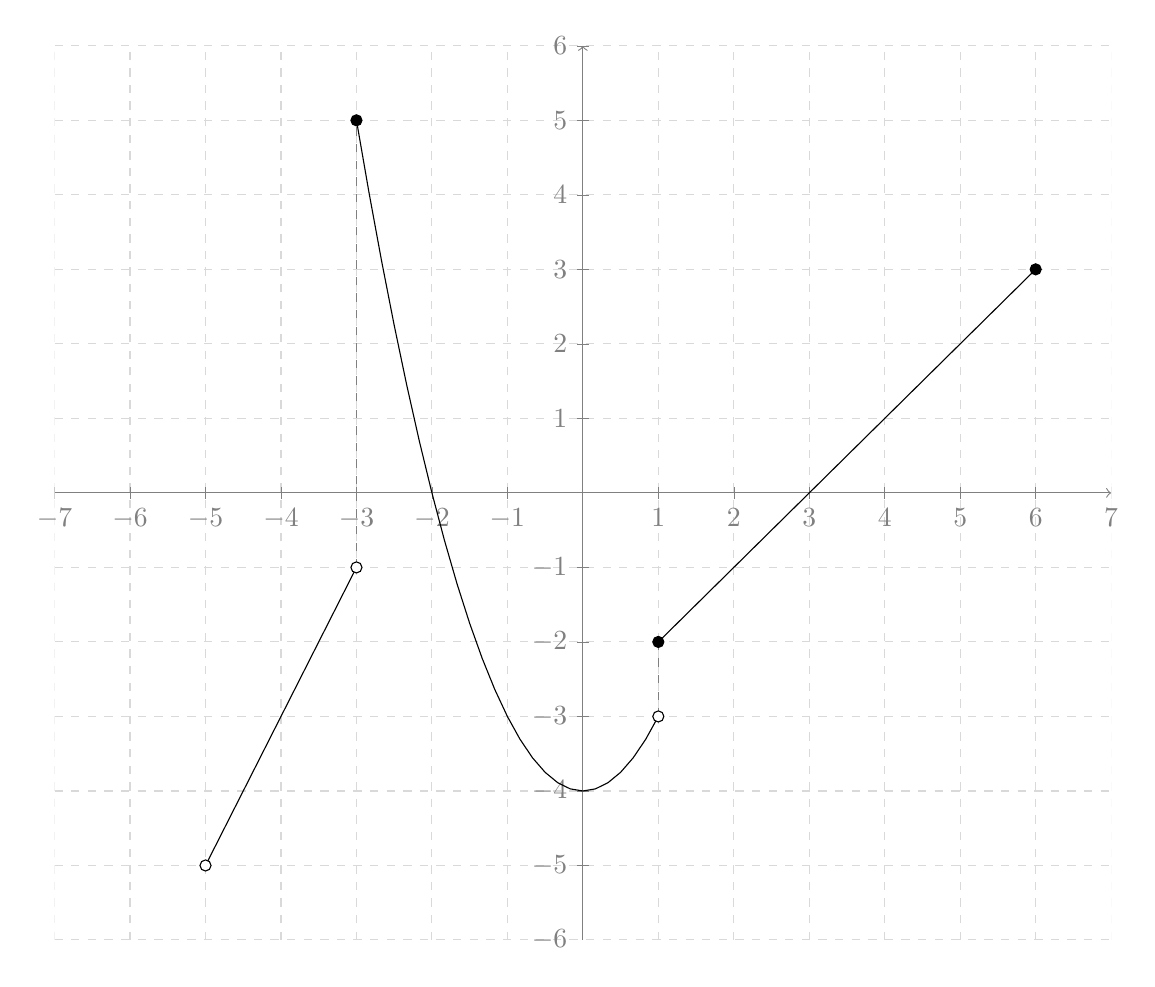
\begin{tikzpicture}[scale=1]
        \begin{axis}[
                %title={$f(x)=x^2-10$},
                axis lines=middle,
                axis line style={->},
                legend style={inner ysep=7pt},
                %x label style={at={(axis description cs:0.5,-0.06)},anchor=north},
                %y label style={at={(axis description cs:-0.06,.5)},rotate=90,anchor=south},
                %xlabel={Nº de bombillas},ylabel={Vida en horas},
                black!50,
                no markers,
                grid,
                width=15cm,
                xmax=7,ymax=6,xmin=-7,ymin=-6,
                %axis lines=middle
                % restrict y to domain=-20:20
            ]
            \addplot[domain=-5:-3,black] {2*x+5};
            \addplot[domain=-3:1,black] {x*x-4};
            \addplot[domain=1:6,black] {x-3};
            \draw[dashed] (axis cs:-3,-1) -- (axis cs:-3,5);
            \draw[dashed] (axis cs:1,-3) -- (axis cs:1,-2);
            \addplot[holdotBlack] coordinates{(-5,-5)(-3,-1)(1,-3)};
            \addplot[soldotBlack] coordinates{(-3,5)(1,-2)(6,3)};
        \end{axis}
    \end{tikzpicture}
\end{questions}
\end{document}